\chapter{Curvilinear Coordinates and Intrinsic Frames}
\label{ch:curvilinear}

\begin{chapterintro}
\textbf{Chapter Objectives:} When trajectories exhibit natural geometric symmetries, Cartesian coordinates become cumbersome. In this chapter, you will master the intrinsic Frenet-Serret frame $(\vec{u}_t, \vec{u}_n, \vec{u}_b)$; calculate radii of curvature; and derive the fundamental velocity and acceleration vectors in plane polar, cylindrical, and spherical coordinates.
\end{chapterintro}

\section{The Intrinsic Frame of Frenet-Serret}

\begin{figure}[htbp]
\centering
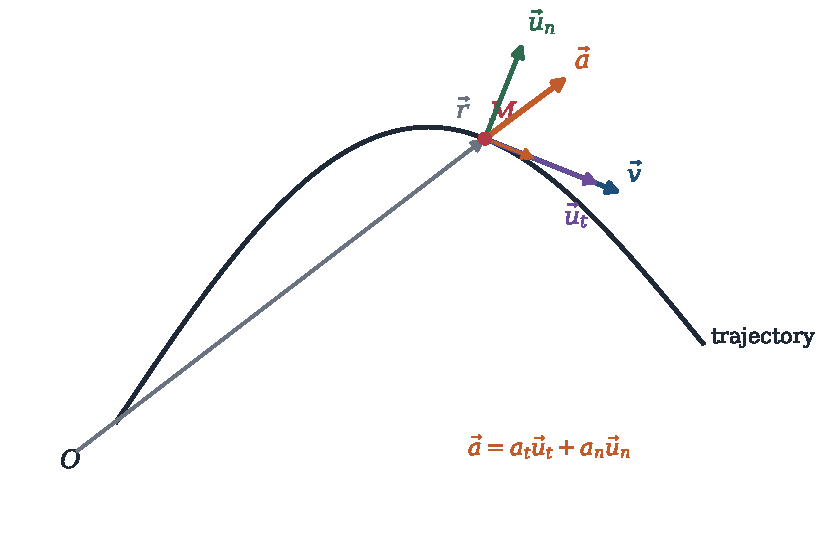
\includegraphics[width=0.74\textwidth]{figures/04_trajectory_frame.pdf}
\caption{The intrinsic Frenet-Serret frame moving along a curved trajectory. Tangent unit vector $\vec{u}_t$ is collinear with velocity, while normal unit vector $\vec{u}_n$ points toward the center of curvature.}
\label{fig:trajectory_frame}
\end{figure}

Let a trajectory curve $\mathcal{C}$ be parametrized by its \textbf{curvilinear abscissa (arc length)} $s(t)$ measured from a reference point $A$:
\[
\dd s = \norm{\dd\vec{r}} = \sqrt{\dd x^2 + \dd y^2 + \dd z^2}.
\]
At any regular point on $\mathcal{C}$, the local moving orthonormal \textbf{Frenet-Serret frame} $(\vec{u}_t, \vec{u}_n, \vec{u}_b)$ is constructed as follows:
\begin{enumerate}[leftmargin=1.5em,itemsep=3pt]
  \item \textbf{Unit Tangent Vector $\vec{u}_t$}:
        \[
        \boxed{\vec{u}_t = \frac{\dd\vec{r}}{\dd s} = \frac{\dd\vec{r}/\dd t}{\dd s/\dd t} = \frac{\vec{v}}{v}.}
        \]
        The velocity is always purely tangential: $\vec{v}(t) = v(t)\,\vec{u}_t$.
  \item \textbf{Unit Principal Normal $\vec{u}_n$ and Radius of Curvature $R$}:
        Since $\vec{u}_t\cdot\vec{u}_t = 1$, its spatial derivative $\frac{\dd\vec{u}_t}{\dd s}$ is strictly orthogonal to $\vec{u}_t$. The \textbf{curvature} $\kappa = 1/R$ and unit principal normal $\vec{u}_n$ are defined by:
        \[
        \boxed{\frac{\dd\vec{u}_t}{\dd s} = \kappa\,\vec{u}_n = \frac{1}{R}\,\vec{u}_n,}
        \]
        where $R$ is the local \textbf{radius of curvature} of the trajectory and $\vec{u}_n$ points into the concave side toward the center of curvature.
  \item \textbf{Unit Binormal Vector $\vec{u}_b$}:
        \[
        \vec{u}_b = \vec{u}_t\times\vec{u}_n.
        \]
\end{enumerate}

\begin{lawbox}{Acceleration in the Frenet-Serret Frame}
Differentiating the velocity $\vec{v} = v\,\vec{u}_t$ with respect to time using the chain rule $\frac{\dd\vec{u}_t}{\dd t} = \frac{\dd s}{\dd t}\frac{\dd\vec{u}_t}{\dd s} = v\left(\frac{1}{R}\vec{u}_n\right)$:
\[
\vec{a}(t) = \frac{\dd}{\dd t}\left(v\,\vec{u}_t\right) = \frac{\dd v}{\dd t}\vec{u}_t + v\frac{\dd\vec{u}_t}{\dd t} = \frac{\dd v}{\dd t}\vec{u}_t + v\left(v\frac{1}{R}\vec{u}_n\right).
\]
Therefore:
\[
\boxed{\vec{a} = a_t\,\vec{u}_t + a_n\,\vec{u}_n = \frac{\dd v}{\dd t}\vec{u}_t + \frac{v^2}{R}\vec{u}_n.}
\]
Notice that the binormal component of acceleration is identically zero ($a_b \equiv 0$); acceleration always lies in the \textbf{osculating plane} spanned by $\vec{u}_t$ and $\vec{u}_n$.
\end{lawbox}

\section{Plane Polar Coordinates $(r, \theta)$}

\begin{figure}[htbp]
\centering
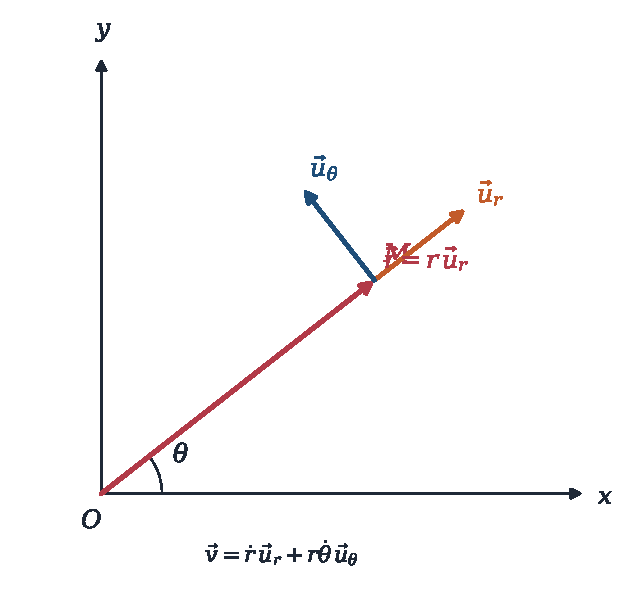
\includegraphics[width=0.74\textwidth]{figures/08_polar_basis.pdf}
\caption{Plane polar basis $(\ur, \ut)$. As the polar angle $\theta$ changes, the unit vectors rotate according to $\dot{\ur} = \dot{\theta}\ut$ and $\dot{\ut} = -\dot{\theta}\ur$.}
\label{fig:polar_basis}
\end{figure}

The position of a particle in the $xy$-plane is specified by radial distance $r = \norm{\vec{OM}}$ and polar angle $\theta$ measured counterclockwise from the positive $x$-axis:
\[
x = r\cos\theta, \qquad y = r\sin\theta.
\]
The orthonormal basis vectors are:
\[
\ur = \cos\theta\,\ihat + \sin\theta\,\jhat, \qquad \ut = -\sin\theta\,\ihat + \cos\theta\,\jhat.
\]
Differentiating with respect to time:
\[
\boxed{\frac{\dd\ur}{\dd t} = \dot{\theta}\,\ut}, \qquad \boxed{\frac{\dd\ut}{\dd t} = -\dot{\theta}\,\ur.}
\]

\begin{lawbox}{Kinematics in Plane Polar Coordinates}
\begin{itemize}[leftmargin=1.4em,itemsep=3pt]
  \item \textbf{Position}:
        \[
        \vec{r} = r\,\ur.
        \]
  \item \textbf{Velocity}:
        \[
        \boxed{\vec{v} = \dot{r}\,\ur + r\dot{\theta}\,\ut = v_r\,\ur + v_\theta\,\ut.}
        \]
  \item \textbf{Acceleration}:
        Differentiating $\vec{v}$:
        \[
        \vec{a} = \ddot{r}\ur + \dot{r}(\dot{\theta}\ut) + \dot{r}\dot{\theta}\ut + r\ddot{\theta}\ut + r\dot{\theta}(-\dot{\theta}\ur).
        \]
        Grouping components:
        \[
        \boxed{\vec{a} = (\ddot{r} - r\dot{\theta}^2)\ur + (r\ddot{\theta} + 2\dot{r}\dot{\theta})\ut = a_r\,\ur + a_\theta\,\ut.}
        \]
        Notice that the transverse component can be written compactly as:
        \[
        \boxed{a_\theta = \frac{1}{r}\frac{\dd}{\dd t}\left(r^2\dot{\theta}\right).}
        \]
        The term $-r\dot{\theta}^2$ is the centripetal acceleration, while $2\dot{r}\dot{\theta}$ is the kinematic \textbf{Coriolis term} in polar coordinates.
\end{itemize}
\end{lawbox}

\section{Cylindrical and Spherical Coordinates}

\begin{figure}[htbp]
\centering
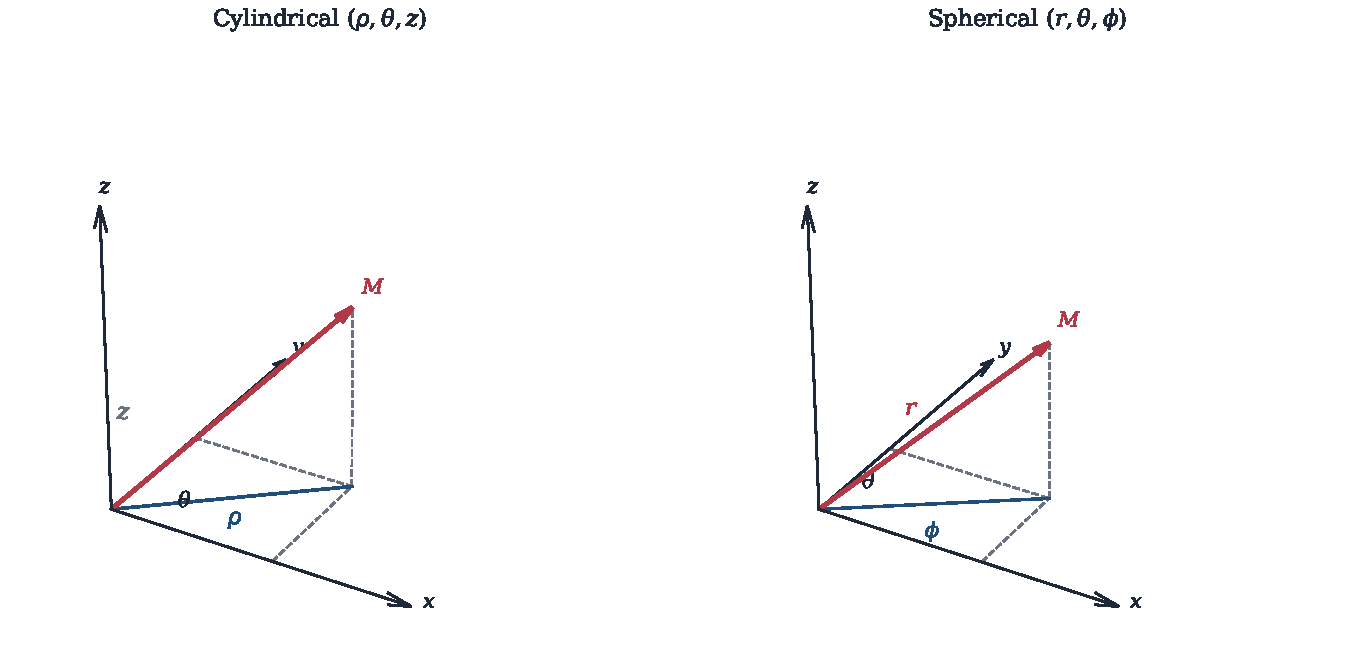
\includegraphics[width=0.82\textwidth]{figures/09_cyl_spherical.pdf}
\caption{Cylindrical coordinates $(\rho, \theta, z)$ and Spherical coordinates $(r, \theta, \phi)$ with their respective local moving coordinate frames.}
\label{fig:cyl_spherical}
\end{figure}

\subsection{Cylindrical Coordinates $(\rho, \theta, z)$}
\begin{align*}
\vec{r} &= \rho\,\vec{u}_\rho + z\,\khat, \\
\vec{v} &= \dot{\rho}\,\vec{u}_\rho + \rho\dot{\theta}\,\ut + \dot{z}\,\khat, \\
\vec{a} &= (\ddot{\rho} - \rho\dot{\theta}^2)\vec{u}_\rho + \frac{1}{\rho}\frac{\dd(\rho^2\dot{\theta})}{\dd t}\ut + \ddot{z}\,\khat.
\end{align*}

\subsection{Spherical Coordinates $(r, \theta, \phi)$}
Here $r \ge 0$ is the radial distance, $\theta \in [0, \pi]$ is the colatitude (polar angle from $+z$), and $\phi \in [0, 2\pi)$ is the azimuthal angle:
\[
x = r\sin\theta\cos\phi, \qquad y = r\sin\theta\sin\phi, \qquad z = r\cos\theta.
\]
The velocity vector is:
\[
\boxed{\vec{v} = \dot{r}\,\ur + r\dot{\theta}\,\ut + r\sin\theta\dot{\phi}\,\uphi.}
\]
The acceleration vector components are:
\begin{align}
a_r &= \ddot{r} - r\dot{\theta}^2 - r\sin^2\theta\dot{\phi}^2, \\
a_\theta &= r\ddot{\theta} + 2\dot{r}\dot{\theta} - r\sin\theta\cos\theta\dot{\phi}^2, \\
a_\phi &= r\sin\theta\ddot{\phi} + 2\sin\theta\dot{r}\dot{\phi} + 2r\cos\theta\dot{\theta}\dot{\phi} = \frac{1}{r\sin\theta}\frac{\dd}{\dd t}\left(r^2\sin^2\theta\dot{\phi}\right).
\end{align}

\section{Extensive Worked Examples}

\begin{workedexample}{Radius of Curvature of a Parabolic Projectile Path}
For a projectile fired with speed $v_0$ at angle $\alpha$, the acceleration is $\vec{a} = -g\jhat$ everywhere.
(a) At the highest point (apex) of the trajectory, find the speed $v_{\text{apex}}$ and the radius of curvature $R_{\text{apex}}$.
(b) At the launch point $(0,0)$, find the tangential acceleration $a_t$ and the radius of curvature $R_{\text{launch}}$.
(c) Deduce the general formula for the radius of curvature $R(t)$ at any instant $t$.

\paragraph{Solution.}

(a) At the apex, the vertical velocity is zero ($v_y = 0$). The velocity is purely horizontal:
\[
\vec{v}_{\text{apex}} = (v_0\cos\alpha)\ihat \implies v_{\text{apex}} = v_0\cos\alpha.
\]
Since velocity is horizontal, the unit tangent is $\vec{u}_t = \ihat$.
The acceleration is purely vertical: $\vec{a} = -g\jhat$.
Because $\vec{a}\perp\vec{v}$, the tangential acceleration is zero: $a_t = 0$.
The entire acceleration is normal (centripetal):
\[
a_n = g.
\]
From the Frenet acceleration relation $a_n = \frac{v^2}{R}$:
\[
g = \frac{v_{\text{apex}}^2}{R_{\text{apex}}} \implies \boxed{R_{\text{apex}} = \frac{v_{\text{apex}}^2}{g} = \frac{v_0^2\cos^2\alpha}{g}.}
\]

(b) At the launch point:
The initial velocity is $\vec{v}_0 = v_0\cos\alpha\,\ihat + v_0\sin\alpha\,\jhat$, with speed $v_0$.
The unit tangent vector is:
\[
\vec{u}_t = \cos\alpha\,\ihat + \sin\alpha\,\jhat.
\]
The tangential acceleration is the projection of $\vec{a} = -g\jhat$ onto $\vec{u}_t$:
\[
a_t = \vec{a}\cdot\vec{u}_t = (-g\jhat)\cdot(\cos\alpha\,\ihat + \sin\alpha\,\jhat) = \boxed{-g\sin\alpha.}
\]
The normal acceleration is obtained from $a^2 = a_t^2 + a_n^2$:
\[
a_n = \sqrt{a^2 - a_t^2} = \sqrt{g^2 - (-g\sin\alpha)^2} = g\sqrt{1 - \sin^2\alpha} = \boxed{g\cos\alpha.}
\]
The radius of curvature at launch is:
\[
a_n = \frac{v_0^2}{R_{\text{launch}}} \implies \boxed{R_{\text{launch}} = \frac{v_0^2}{a_n} = \frac{v_0^2}{g\cos\alpha}.}
\]

(c) At any arbitrary instant $t$:
The speed is $v(t) = \sqrt{(v_0\cos\alpha)^2 + (v_0\sin\alpha - gt)^2}$.
The cross product $\norm{\vec{v}\times\vec{a}}$ provides an elegant shortcut:
\[
\vec{v}\times\vec{a} = (v_x\ihat + v_y\jhat)\times(-g\jhat) = -g v_x\,\khat \implies \norm{\vec{v}\times\vec{a}} = g v_x = g v_0\cos\alpha.
\]
On the other hand, in the Frenet frame $\vec{v} = v\vec{u}_t$ and $\vec{a} = a_t\vec{u}_t + a_n\vec{u}_n$:
\[
\norm{\vec{v}\times\vec{a}} = \norm{v\vec{u}_t\times(a_t\vec{u}_t + a_n\vec{u}_n)} = v a_n = v\left(\frac{v^2}{R}\right) = \frac{v^3}{R}.
\]
Equating the two expressions:
\[
\frac{v^3}{R} = g v_0\cos\alpha \implies \boxed{R(t) = \frac{v^3(t)}{g v_0\cos\alpha} = \frac{\left[ (v_0\cos\alpha)^2 + (v_0\sin\alpha - gt)^2 \right]^{3/2}}{g v_0\cos\alpha}.}
\]
At $t = 0$, $R(0) = \frac{v_0^3}{g v_0\cos\alpha} = \frac{v_0^2}{g\cos\alpha}$; at apex ($v_y = 0$), $R = \frac{(v_0\cos\alpha)^3}{g v_0\cos\alpha} = \frac{v_0^2\cos^2\alpha}{g}$. Exact agreement!
\end{workedexample}

\begin{workedexample}{Particle Moving on a Circular Helix}
A particle moves along a vertical circular helix of radius $R$ and pitch $2\pi h$ according to:
\[
\vec{r}(t) = R\cos(\omega t)\,\ihat + R\sin(\omega t)\,\jhat + (c\omega t)\,\khat,
\]
where $\omega$ and $c$ are positive constants.
(a) Find the velocity vector $\vec{v}(t)$ and speed $v$.
(b) Determine the Frenet unit vectors $\vec{u}_t, \vec{u}_n, \vec{u}_b$.
(c) Calculate the radius of curvature $R_c$ and the torsion $\tau$ of the helix.

\paragraph{Solution.}

(a) Differentiating position with respect to time:
\[
\vec{v}(t) = \dot{\vec{r}}(t) = -R\omega\sin(\omega t)\,\ihat + R\omega\cos(\omega t)\,\jhat + c\omega\,\khat.
\]
The speed is constant:
\[
\boxed{v = \norm{\vec{v}} = \sqrt{(-R\omega\sin\omega t)^2 + (R\omega\cos\omega t)^2 + (c\omega)^2} = \omega\sqrt{R^2 + c^2} = \text{const}.}
\]

(b) Frenet vectors:
\begin{itemize}[leftmargin=1.4em,itemsep=2pt]
  \item Unit tangent:
  \[
  \vec{u}_t = \frac{\vec{v}}{v} = \frac{1}{\sqrt{R^2 + c^2}}\left[ -R\sin(\omega t)\,\ihat + R\cos(\omega t)\,\jhat + c\,\khat \right].
  \]
  \item Acceleration:
  \[
  \vec{a}(t) = \dot{\vec{v}}(t) = -R\omega^2\cos(\omega t)\,\ihat - R\omega^2\sin(\omega t)\,\jhat + 0\,\khat = -R\omega^2\left[ \cos(\omega t)\,\ihat + \sin(\omega t)\,\jhat \right].
  \]
  Since speed is constant ($v = \text{const}$), the tangential acceleration is zero: $a_t = \dot{v} = 0$.
  Thus $\vec{a} = a_n\vec{u}_n$. Since $\norm{\vec{a}} = R\omega^2$, the unit principal normal is:
  \[
  \vec{u}_n = \frac{\vec{a}}{\norm{\vec{a}}} = \boxed{-\cos(\omega t)\,\ihat - \sin(\omega t)\,\jhat.}
  \]
  The principal normal points horizontally directly toward the central axis of the cylinder!
  \item Unit binormal:
  \begin{align*}
  \vec{u}_b &= \vec{u}_t\times\vec{u}_n = \frac{1}{\sqrt{R^2 + c^2}}\begin{vmatrix} \ihat & \jhat & \khat \\ -R\sin\omega t & R\cos\omega t & c \\ -\cos\omega t & -\sin\omega t & 0 \end{vmatrix} \\
  &= \frac{1}{\sqrt{R^2 + c^2}}\left[ c\sin(\omega t)\,\ihat - c\cos(\omega t)\,\jhat + (R\sin^2\omega t + R\cos^2\omega t)\khat \right] \\
  &= \boxed{\frac{1}{\sqrt{R^2 + c^2}}\left[ c\sin(\omega t)\,\ihat - c\cos(\omega t)\,\jhat + R\,\khat \right].}
  \end{align*}
\end{itemize}

(c) Curvature and radius of curvature:
\[
a_n = \frac{v^2}{R_c} \implies R\omega^2 = \frac{\omega^2(R^2 + c^2)}{R_c} \implies \boxed{R_c = \frac{R^2 + c^2}{R} = R\left(1 + \frac{c^2}{R^2}\right).}
\]
Notice that $R_c > R$: the curvature of a helix is always strictly less than the curvature of its base circle!

For torsion $\tau$: from the third Frenet-Serret formula $\frac{\dd\vec{u}_b}{\dd s} = -\tau\vec{u}_n$:
\[
\frac{\dd\vec{u}_b}{\dd t} = \frac{c\omega}{\sqrt{R^2 + c^2}}\left[ \cos(\omega t)\,\ihat + \sin(\omega t)\,\jhat \right] = -\frac{c\omega}{\sqrt{R^2 + c^2}}\vec{u}_n.
\]
Since $\frac{\dd\vec{u}_b}{\dd t} = v\frac{\dd\vec{u}_b}{\dd s} = -v\tau\vec{u}_n$:
\[
v\tau = \frac{c\omega}{\sqrt{R^2 + c^2}} \implies \left(\omega\sqrt{R^2 + c^2}\right)\tau = \frac{c\omega}{\sqrt{R^2 + c^2}} \implies \boxed{\tau = \frac{c}{R^2 + c^2}.}
\]
Both the curvature and the torsion of a circular helix are constant everywhere along its length.
\end{workedexample}
